\documentclass{beamer}[10]

\usepackage{graphicx}
\usepackage{xcolor}
\usepackage{tabto}
%\usepackage{beamerthemesplit}
\usepackage{tikz}
\usepackage{cancel}
\usepackage{verbatim}
\usepackage{fancybox}
\usepackage{enumerate}
\usepackage{amsmath,amssymb,amsthm,textcomp,mathtools}
\usepackage[super]{nth}
\usepackage[amssymb]{SIunits}
\usepackage{booktabs}
\usepackage{cancel}
\usepackage{bm}
\usepackage[utf8]{inputenc}
\usepackage{tabularx}
\usepackage{ragged2e}
\newcolumntype{Y}{ >{\RaggedRight\arraybackslash}X}
\usetikzlibrary{arrows,shapes}
\newcommand\T{\rule{0pt}{2.6ex}}
\newcommand\B{\rule[-1.2ex]{0pt}{0pt}}
\definecolor{UUcrimson}{RGB}{204,0,0}
\mode<presentation>
{ \usetheme{default}
  \usecolortheme[named=UUcrimson]{structure}
  \useinnertheme{circles}
  \setbeamercovered{transparent}
  \setbeamertemplate{blocks}[rounded]
  \usefonttheme[onlymath]{serif}
  \setbeamertemplate{navigation symbols}{}
  \setbeamertemplate{footline}[page number]
  \setbeamertemplate{navigation symbols}{}
  \setbeamercolor{section in toc}{fg=black,bg=white}
  \setbeamercolor{alerted text}{fg=UUcrimson!80!gray}
  \setbeamercolor*{palette primary}{fg=white,bg=UUcrimson}
  \setbeamercolor*{palette secondary}{fg=UUcrimson!70!black,bg=gray!15!white}
  \setbeamercolor*{palette tertiary}{bg=UUcrimson!80!black,fg=gray!10!white}
  \setbeamercolor*{palette quaternary}{fg=UUcrimson,bg=gray!5!white}
  \setbeamercolor*{palette sidebar primary}{fg=UUcrimson!10!black}
  \setbeamercolor*{palette sidebar secondary}{fg=white}
  \setbeamercolor*{palette sidebar tertiary}{fg=UUcrimson!50!black}
  \setbeamercolor*{palette sidebar quaternary}{fg=gray!10!white}
  \setbeamercolor{titlelike}{parent=palette primary,fg=white}
  \setbeamercolor{frametitle}{bg=UUcrimson}
  \setbeamercolor{frametitle right}{bg=UUcrimson}
  \setbeamercolor*{separation line}{}
  \setbeamercolor*{fine separation line}{}
}

\usetikzlibrary{backgrounds}
\makeatletter
\tikzstyle{every picture}+=[remember picture]
\tikzset{%
  fancy quotes/.style={
    text width=\fq@width pt,
    align=justify,
    inner sep=1em,
    anchor=north west,
    minimum width=\linewidth,
    font=\itshape
  },
  fancy quotes width/.initial={.8\linewidth},
  fancy quotes marks/.style={
    scale=8,
    text=white,
    inner sep=0pt,
  },
  fancy quotes opening/.style={
    fancy quotes marks,
  },
  fancy quotes closing/.style={
    fancy quotes marks,
  },
  fancy quotes background/.style={
    show background rectangle,
    inner frame xsep=0pt,
    background rectangle/.style={
      fill=gray!25,
      rounded corners,
    },
  }
}
\newenvironment{fancyquotes}[1][]{%
\noindent
\tikzpicture[fancy quotes background]
\node[fancy quotes opening,anchor=north west] (fq@ul) at (0,0) {``};
\tikz@scan@one@point\pgfutil@firstofone(fq@ul.east)
\pgfmathsetmacro{\fq@width}{\linewidth - 2*\pgf@x}
\node[fancy quotes,#1] (fq@txt) at (fq@ul.north west) \bgroup}
{\egroup;
\node[overlay,fancy quotes closing,anchor=east] at (fq@txt.south east) {''};
\endtikzpicture}
\makeatother

\usepackage{scalerel}[2014/03/10]
\usepackage{stackengine}
\usepackage{empheq}
\newcommand*\widefbox[1]{\fbox{\hspace{0.5em}#1\hspace{0.5em}}}

\newcommand\reallywidetilde[1]{\ThisStyle{%
  \setbox0=\hbox{$\SavedStyle#1$}%
  \stackengine{-.1\LMpt}{$\SavedStyle#1$}{%
    \stretchto{\scaleto{\SavedStyle\mkern.2mu\sim}{.5467\wd0}}{.4\ht0}%
%    .2mu is the kern imbalance when clipping white space
%    .5467++++ is \ht/[kerned \wd] aspect ratio for \sim glyph
  }{O}{c}{F}{T}{S}%
}}
\usepackage{media9}

\logo{
\includegraphics[width=0.75cm]{logo.jpg}}
\author[Gibbs]{Dr. Jeremy A. Gibbs}
\institute{Department of Mechanical Engineering\\University of Utah}
\date{Fall 2016}
\title{LES of Turbulent Flows: Lecture 13}

\begin{document}

%----------------------------------------------------------------------------------------
%	TITLE & TOC SLIDES
%----------------------------------------------------------------------------------------

\begin{frame} 
  \titlepage
\end{frame}

%------------------------------------------------

\begin{frame}
\frametitle{Overview}
\tableofcontents
\end{frame}

%------------------------------------------------
\section{Recap: Eddy-Viscosity Models} %
%------------------------------------------------
\begin{frame}{Eddy-Viscosity Models}
\begin{itemize}
	\item In Lecture 12 we said that eddy-viscosity models are of the form:
	\begin{align*}
		\text{momentum} \qquad \tau_{ij} &= -2\nu_{T} \widetilde{S}_{ij}\\
		\text{scalars} \qquad q_i &= -D_T \frac{\partial \widetilde{\theta}}{\partial x_i}
	\end{align*}
	where
	$$D_T = \frac{\nu_T}{\text{Pr}},$$
	\item $\widetilde{S}_{ij}$ is the filtered strain rate
	\item $\nu_T$ is eddy-viscosity
	\item $D_T$ is eddy-diffusivity
	\item Pr is the SGS Prandtl number 
\end{itemize}

\end{frame}

%------------------------------------------------
\begin{frame}{Eddy-Viscosity Models}
\begin{itemize}
	\item This is the LES equivalent to \nth{1}-order RANS closure (k-theory or gradient transport theory) and is an analogy to molecular viscosity
	\item Turbulent fluxes are assumed to be proportional to the local velocity or scalar gradients
	\item In LES, this is the assumption that stress is proportional to strain: $\tau_{ij} \sim \widetilde{S}_{ij}$
	\item The SGS eddy-viscosity $\nu_T$ must be parameterized   
\end{itemize}

\end{frame}

%------------------------------------------------
\begin{frame}{Eddy-Viscosity Models}
\begin{itemize}
	\item Dimensionally
	$$\nu_T = \left[ \frac{L^2}{T}\right]$$
	\item In almost all SGS eddy-viscosity models:
	$$\nu_T \sim U\ell$$
	\item Different models use different $U$ and $\ell$
\end{itemize}

\end{frame}

%------------------------------------------------

\begin{frame}{Eddy-Viscosity Models}

\textbf{Interpretation}
\begin{itemize}
	\item Recall that we can interpret the eddy-viscosity as adding to the molecular viscosity.
	$$2\frac{\partial}{\partial x_j}\left[\left(\nu_T + \nu\right)\widetilde{S}_{ij}\right]$$	
\end{itemize}

\textbf{What does the model do?}
\begin{itemize}
	\item We can see it effectively lowers the Reynolds number of the flow
	\item It provides all of the energy dissipation for high Re flows (when 1/Re$\Rightarrow$0).
\end{itemize}
\end{frame}

%------------------------------------------------
\section{Smagorinsky Model} %
%------------------------------------------------
\begin{frame}{Smagorinsky Model}
\begin{itemize}
	\item One of the first and most popular eddy-viscosity models for LES is the Smagorinsky model (Smagorinsky 1963)
	\item The model was originally developed for general circulation (large-scale atmospheric) models
	\item The model did not remove enough energy in this context
\end{itemize}

\end{frame}

%------------------------------------------------
\begin{frame}{Smagorinsky Model}
\begin{itemize}
	\item The Smagorinsky model was applied by Deardorff (1970) in the first reported LES
	\item Deardorff used Prandtl’s mixing length idea (1925) applied at the SGSs (see Pope Ch. 10 or Stull, 1988 for a full review of mixing length)
\end{itemize}

\end{frame}

%------------------------------------------------
\begin{frame}{Smagorinsky Model}
\textbf{Prandtl's mixing length} -- for a general scalar quantity $q$ with an assumed linear profile:

\begin{columns}[T]
	\begin{column}{.26\textwidth}
    	\begin{minipage}[c][.5\textheight][c]{\linewidth}
    		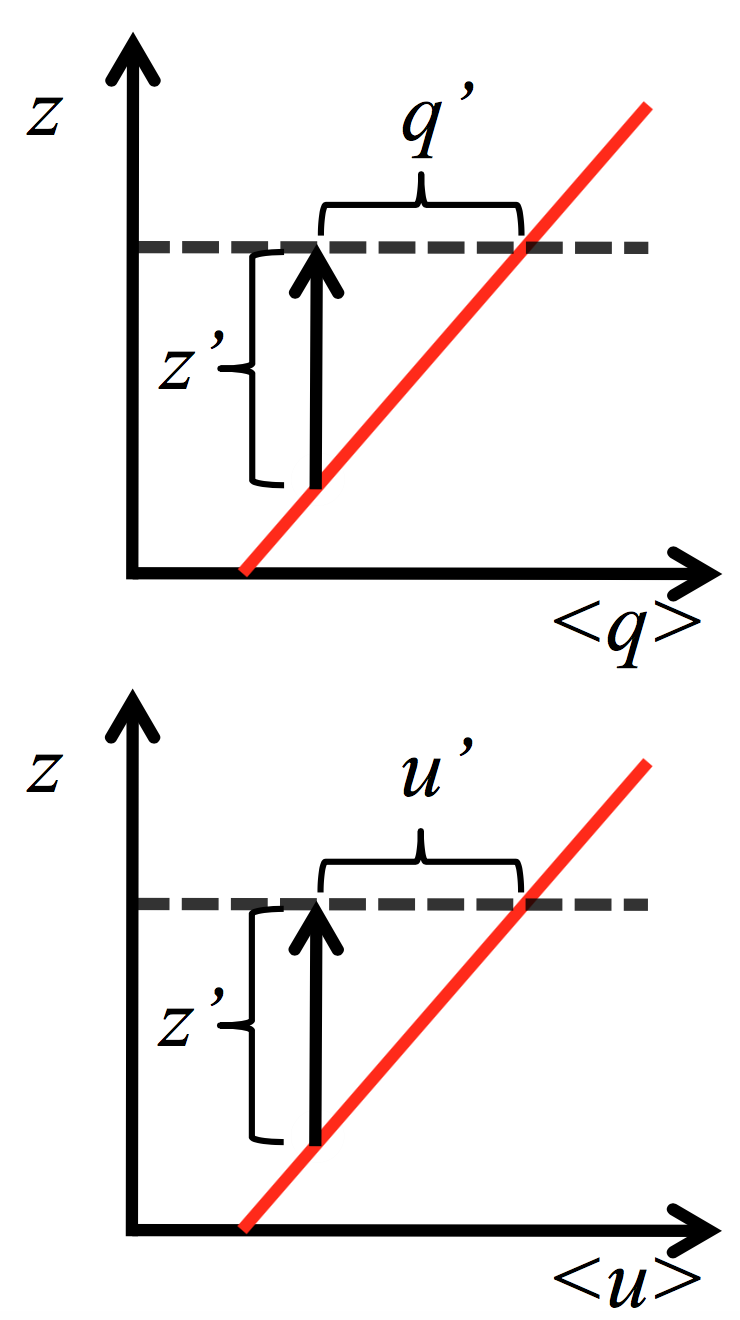
\includegraphics[width=1\textwidth]{mixing_length}
    	\end{minipage}
    \end{column}
    \begin{column}{.74\textwidth}
    	\begin{itemize}
    		\item A turbulent eddy moves a parcel of air by an amount $z^\prime$ towards a level $z$ where we have no mixing or other change
    		\item $q$ will differ from the surrounding air by:
    		$$q^\prime = -\left(\frac{\partial \langle q\rangle}{\partial z}\right)z^\prime$$
    		\textit{i.e.}, the scalar will change proportional to its local gradient
    	\end{itemize}	
    \end{column}
  \end{columns}

\end{frame}

%------------------------------------------------
\begin{frame}{Smagorinsky Model}
\textbf{Prandtl's mixing length} -- likewise, for velocity $u$ with an assumed linear profile:

\begin{columns}[T]
	\begin{column}{.26\textwidth}
    	\begin{minipage}[c][.5\textheight][c]{\linewidth}
    		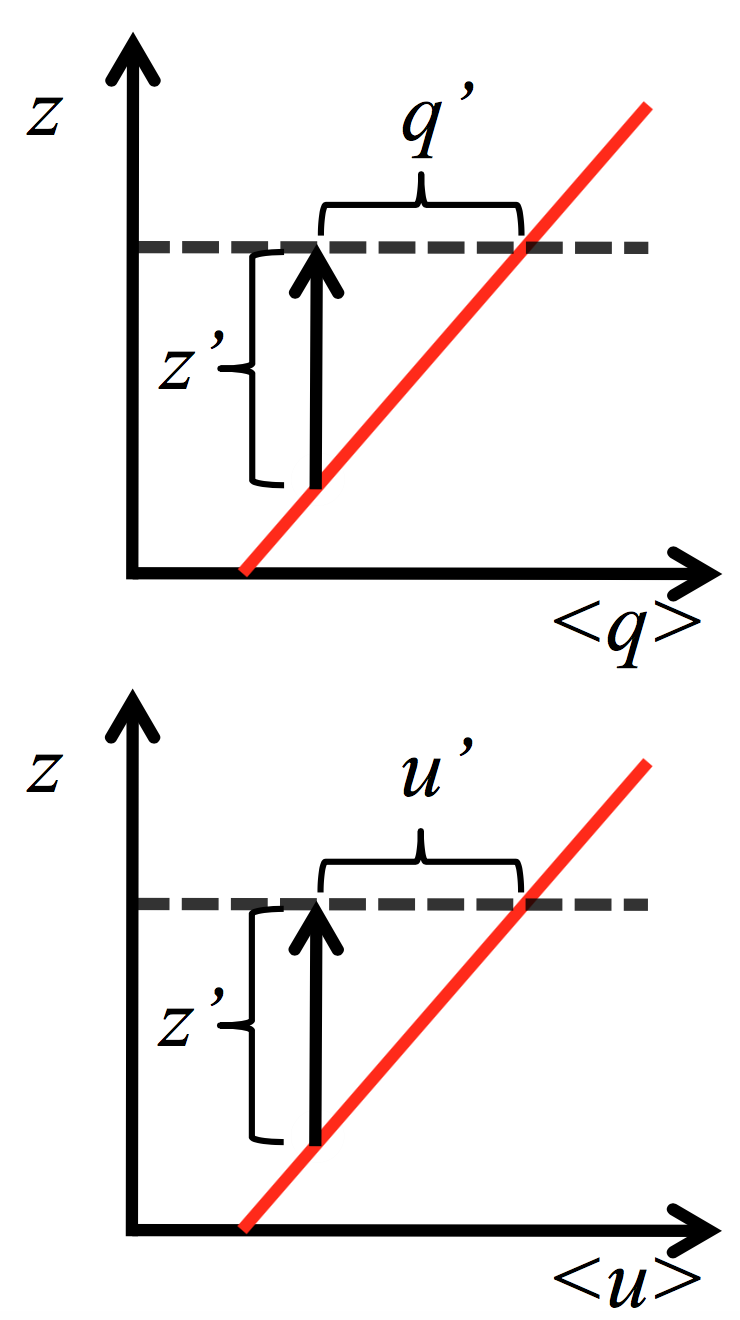
\includegraphics[width=1\textwidth]{mixing_length}
    	\end{minipage}
    \end{column}
    \begin{column}{.74\textwidth}
    	\begin{itemize}
    		\item A turbulent eddy moves a parcel of air by an amount $z^\prime$ towards a level $z$ where we have no mixing or other change
    		\item $u$ will differ from the surrounding air by:
    		$$u^\prime = -\left(\frac{\partial \langle u\rangle}{\partial z}\right)z^\prime$$
    		\textit{i.e.}, the velocity will change proportional to its local gradient
    	\end{itemize}	
    \end{column}
  \end{columns}

\end{frame}

%------------------------------------------------
\begin{frame}{Smagorinsky Model}
\textbf{Prandtl's mixing length}

\begin{itemize}
	\item In order to move up a distance $z^\prime$, our air parcel must have some vertical velocity $w^\prime$
	\item If turbulence is such that $w^\prime \propto u^\prime$, then $w^\prime = Cu^\prime$
	\item We have two cases:
	\begin{align*}
	\frac{\partial u}{\partial z} &> 0 \Rightarrow w^\prime = -Cu^\prime\\\\
	\frac{\partial u}{\partial z} &< 0 \Rightarrow w^\prime = Cu^\prime	
	\end{align*}
	\item Combining these, we get that:
	$$w^\prime = C \left| \frac{\partial \langle u\rangle}{\partial z}\right|z^\prime$$
\end{itemize}

\end{frame}

%------------------------------------------------
\begin{frame}{Smagorinsky Model}
\textbf{Prandtl's mixing length}

\begin{itemize}
	\item We now have:
	\begin{align*}
		q^\prime &= -\left(\frac{\partial \langle q\rangle}{\partial z}\right)z^\prime\\
		w^\prime &= C \left| \frac{\partial \langle u\rangle}{\partial z}\right|z^\prime
	\end{align*}
	\item We can form a kinematic flux (conc. * velocity) by multiplying the two together:
	$$\langle w^\prime q^\prime \rangle = -C\langle (z^\prime)^2 \rangle \left| \frac{\partial \langle u\rangle}{\partial z}\right| \frac{\partial \langle q\rangle}{\partial z}$$
\end{itemize}

\end{frame}

%------------------------------------------------
\begin{frame}{Smagorinsky Model}
\textbf{Prandtl's mixing length}

\begin{itemize}
	\item Prandtl assumed that the constant of proportionality is unity and called $z^\prime$ the mixing length ($\ell$)  
	$$\langle w^\prime q^\prime \rangle = -\ell^2 \left| \frac{\partial \langle u\rangle}{\partial z}\right| \frac{\partial \langle q\rangle}{\partial z}$$
	\item We can replace $q^\prime$ with any variable in this relationship \\(\textit{e.g.}, $u^\prime$)
	\item You can think of $(z^\prime)^2$ or $\ell^2$ as the variance of a parcel's movement 
\end{itemize}

\end{frame}

%------------------------------------------------
\begin{frame}{Smagorinsky Model}
\textbf{Prandtl's mixing length} - what is it? Let's ask Prandtl.

	\begin{fancyquotes}
		may be considered as the diameter of the masses of fluid moving as a whole in each individual case; or again, as the distance traversed by a mass of this type before it becomes blended in with neighbouring masses\\ \ldots \\
		somewhat similar, as regards effect, to the mean free path in the kinetic theory of gases\\ \ldots \\
		only a rough approximation
	\end{fancyquotes}
In other words, the mixing length according to Prandtl is the average distance that a fluid mass will travel before it is changed by the new environment
\end{frame}

%------------------------------------------------
\begin{frame}{Smagorinsky Model}
\textbf{Back to the Smagorinsky model}

Recall:
\begin{itemize}
	\item Dimensionally
	$$\nu_T = \left[ \frac{L^2}{T}\right]$$
	\item In almost all SGS eddy-viscosity models:
	$$\nu_T \sim \ell U$$
	\item Different models use different $\ell$ and $U$
\end{itemize}

\begin{itemize}
	\item Use Prandtl's mixing length applied at the SGSs
	$$\nu_T = \underbrace{(C_S \Delta)^2 | \widetilde{S}|}_{\ell \ell T^{-1}\ =\ \ell U}$$
\end{itemize}

\end{frame}

%------------------------------------------------
\begin{frame}{Smagorinsky Model}
$$\nu_T = (C_S \Delta)^2 | \widetilde{S}|$$

\begin{itemize}
	\item $\Delta = (\Delta_x \Delta_y \Delta_z)^{\frac{1}{3}}$ is the effective grid scale (see Deardorff 1970 or Scotti et al, 1993)
	\item $C_S \Delta$ is the length scale -- squared for dimensional consistency
	\item $|\widetilde{S}| = \sqrt{2\widetilde{S}_{ij}\widetilde{S}_{ij}}$ is the magnitude of the filtered strain rate tensor with units of [$T^{-1}$]. It serves as part of the velocity scale -- think $\partial \langle u \rangle / \partial z$ in Prandtl's theory
\end{itemize}

\end{frame}

%------------------------------------------------
\begin{frame}{Smagorinsky Model}

\begin{itemize}
	\item The final model is 
	$$\tau_{ij} - \frac{1}{3}\tau_{kk}\delta_{ij} = -2\nu_{T} \widetilde{S}_{ij} = -2 (C_S \Delta)^2 | \widetilde{S}| \widetilde{S}_{ij}$$
	\item In order to close the model, we need a value of $C_S$ (usually called the Smagorinsky or Smagorinsky-Lilly coefficient)
\end{itemize}

\end{frame}

%------------------------------------------------
\begin{frame}{Smagorinsky Model}

\begin{itemize}
	\item Lilly (1967) proposed a method to determine $C_S$ (see also Pope pg 587)
	\item We assume that we have a high-Re flow such that $\Delta$ can be taken to be in the inertial subrange of turbulence
	\item The mean energy transfer across $\Delta$ must be balanced, on average,  by viscous dissipation (note: for $\Delta$ in the inertial subrange this is not an assumption)
	\begin{align*}
		\epsilon &= \langle \Pi \rangle\\
		\text{recall:}\qquad \Pi &= -\tau_{ij} \widetilde{S}_{ij}
	\end{align*}
	
\end{itemize}

\end{frame}

%------------------------------------------------
\begin{frame}{Smagorinsky Model}

\begin{itemize}
	\item Using an eddy-viscosity model, we get
	$$\Pi = -\tau_{ij} \widetilde{S}_{ij} = 2\nu_T \widetilde{S}_{ij}\widetilde{S}_{ij} = \nu_T |\widetilde{S}|^2$$
	\item We can use the Smagorinsky model
	$$\nu_T = (C_S \Delta)^2 | \widetilde{S}|$$
	to arrive at:
	$$\Pi = (C_S \Delta)^2 | \widetilde{S}|^3$$
\end{itemize}

\end{frame}

%------------------------------------------------
\begin{frame}{Smagorinsky Model}

\begin{itemize}
	\item The square of $|\widetilde{S}|$ can be written as (see Liily 1967 and Pope pg 579):
	$$|\widetilde{S}|^2 = 2\int^{\infty}_{0} k^2 \hat G(k)^2 E(k) dk$$
	where $\hat(G)(k)$ is the filter transfer function and $E(k)$ is the energy spectrum
	\item Recall that for a Kolmogorov spectrum in the inertial subrange:
	$$E(k) \sim C_k \epsilon^\frac{2}{3}k^{-\frac{5}{3}}$$
\end{itemize}

\end{frame}

%------------------------------------------------
\begin{frame}{Smagorinsky Model}

\begin{itemize}
	\item Substitution of the Kolmogorov $E(k)$ yields
	\begin{align*}
		|\widetilde{S}|^2 &= 2\int^{\infty}_{0} k^2 \hat G(k)^2 E(k) dk \approx 2\int^{\infty}_{0} k^2 \hat G(k)^2 C_k \epsilon^\frac{2}{3} k^{-\frac{5}{3}} dk\\ 
		&\approx a_f C_k \epsilon^\frac{2}{3} \Delta^{-\frac{4}{3}}
	\end{align*}
	where
	$$a_f = 2\int^{\infty}_{0} (k\Delta)^{\frac{1}{3}} \hat G(k)^2 \Delta dk$$ 
	Note that $a_f$ depends on the filter, but is independent of $\Delta$
\end{itemize}

\end{frame}

%------------------------------------------------
\begin{frame}{Smagorinsky Model}

\begin{itemize}
	\item We can rearrange $|\widetilde{S}|^2 = a_f C_k \epsilon^\frac{2}{3} \Delta^{-\frac{4}{3}}$ to get:
	$$\epsilon = \left[ \frac{\langle|\widetilde{S}|^2\rangle}{a_f C_k \Delta^{-\frac{4}{3}}}\right]^{\frac{3}{2}}$$
	\item Recall that we are equating viscous dissipation and the average Smagorinsky SGS dissipation:
	$$\epsilon = \langle \Pi \rangle$$
	where 
	$$\Pi = (C_S \Delta)^2 | \widetilde{S}|^3$$
\end{itemize}

\end{frame}

%------------------------------------------------
\begin{frame}{Smagorinsky Model}

\begin{itemize}
	\item Combining these expression yields:
	$$ (C_S \Delta)^2 \langle| \widetilde{S}|^3 \rangle = \left[ \frac{\langle|\widetilde{S}|^2\rangle}{a_f C_k \Delta^{-\frac{4}{3}}}\right]^{\frac{3}{2}}$$
	Algebra then gives us:
	$$C_S = \frac{1}{(a_f C_k)^{3/4}}\left(\frac{\langle |\widetilde{S}_{ij}|^3 \rangle}{\langle |\widetilde{S}_{ij}|^2\rangle^{3/2}}\right)^{-\frac{1}{2}}$$
\end{itemize}

\end{frame}

%------------------------------------------------
\begin{frame}{Smagorinsky Model}

\begin{itemize}
	\item We can approximate that $\langle |\widetilde{S}_{ij}|^2\rangle^{3/2} \approx \langle |\widetilde{S}_{ij}|^3 \rangle$
	\item We can also make use of $a_f =(3/2\pi)^{4/3}$ for a sharp cutoff filter (see Pope)
	\item Substitution yields
	$$C_S = \frac{1}{\pi}\left(\frac{2}{3C_k}\right)^{\frac{3}{4}}$$
	\item $C_k$ is the Kolmogorov ``constant'' and is generally taken as $C_k\approx 1.5$-$1.6$. Using this values leads to
	$$\boxed{C_S \approx 0.17}$$
\end{itemize}

\end{frame}

%------------------------------------------------

\end{document}

